%************************************************
\chapter{Introduction}\label{ch:introduction}
%************************************************
Natural language processing deals with extracting the subjective information from natural language texts.
One such information is the sentiment behind the text. This has also been referred to as opinion/mood/attitude/appraisal/evaluation in the literature.
The simplest form of sentiment analysis involves identifying the polarity of a text, which can be positive, negative or neutral. \vspace{8mm} 

An analysis of this form is very useful when the text is large and manual examination is impossible. For instance, a company can easily obtain a feedback on its newly released
by performing such an analysis on its review page. Note that this kind of feedback is more natural since the customers/reviewers may write more freely when writing a review
in natural language rather than when rating a product numerically (say, on a one to five stars scale) or when filling up feedback forms. More importantly, companies 
don't have to ask their customers for feedback. The customers post feedbacks at their own leisure in their own writing styles. What is needed is a way to automatically analyse all
these reviews and generate some result (may be a numerical score or labels like positive or negative) that may be indicative of the overall customer experience. Sentiment
analysis seeks to provide that way. \vspace{8mm} 

Putting it simply, if we perform sentiment analysis on a movie review page, and there are more posts like \vspace{8mm} \\
\textbf{"Loved the movie! Too good. :)"} \vspace{8mm} \\
and less posts like \vspace{8mm} \\
\textbf{"Boring! Wasted time and money."}, \vspace{8mm} \\  
we should be able to conclude that the movie review document has a positive sentiment. This is the minimal setting for a sentiment analysis problem.

\section{Sentiment Analysis}

Sentiment analysis can be defined as the process of computationally identifying and categorizing sentiments expressed in a piece of text 
to determine whether the attitude of writer (rather, the sentiment holder) towards a particular topic, product, etc. is positive, negative, or neutral.

\subsection{Sentiment analysis research}

Sentiment analysis is a Natural Language Processing (NLP) problem. It touches several aspects of NLP, e.g., coreference resolution, negation handling, and
word sense disambiguation, which makes it a difficult task since these are not solved problems in NLP. However, sentiment analysis is a highly restricted NLP problem 
because the system need not fully understand the semantics the text but
only needs to understand some aspects of it, i.e., positive or negative sentiments and their target entities or topics. \vspace{8mm} 

Sentiment analysis is a relatively new branch of research, having evolved mainly after 2000 AD. However, the research has taken a serious shape since, and 
there is a heavy ongoing research in this area. There are several reasons for this.

\begin{enumerate}[(a)]%for small alpha-characters within brackets.
\item It has a wide arrange of applications, almost in every domain.
\item Commercial applications have proliferated.
\item It offers many challenging research problems, which had never been studied before.
\item Ever since the evolution of the likes of social networks and blogs, data of unprecedented scale is available for analysis.
\end{enumerate}  

Sentiment can be defined as a quintuple:

\begin{framed}
\begin{eqnarray}
 ( e_i , a_{ij} , s_{ijkl} , h_k , t_l ) \nonumber
\end{eqnarray}
\end{framed}

Here,

\begin{itemize}
 \item $e_i$ is the name of an entity
 \item $a_{ij}$ is an aspect of $e_i$
 \item $s_{ijkl}$ is the sentiment on aspect $a_{ij}$ of entity $e_i$
 \item $h_k$ is the opinion holder
 \item $t_l$ is the time when the opinion is expressed by $h_k$
\end{itemize}

Thus, the task of setiment analysis can be stated as:
Given a sentiment document d, discover all sentiment quintuples $( e_i , a_{ij} , s_{ijkl} , h_k , t_l )$ in d. However, it is unlikely that we 
will ever use all of the components of the quintuple in a particular problem. \cite{book}

\subsection{Levels of sentiment analysis}

Sentiment analysis can be performed at many levels: 

\begin{enumerate}[(a)]%for small alpha-characters within brackets.
\setlength{\itemsep}{15pt}
\item \textbf{Document Level: } In this level, we assume that the entire document talks about one particular entity only. 
In this type of a setting, the opinion holder and time are usually irrelevant. Since we are concerned with just one target throughout the text, the aspect is GENERAL.
The opinion tuple thus becomes: 

\begin{framed}
\begin{eqnarray}
 ( e_i , GENERAL , s_{ijkl} , - , - ) \nonumber
\end{eqnarray}
\end{framed}

\item \textbf{Sentence Level: } This level of analysis goes to the sentences to determine whether each sentence is positive, negative or neutral.
\item \textbf{Aspect Level: } It is based on the idea that an opinion/sentiment consists of a sentiment (positive or negative) and a target. This is a fine-grained 
analysis where we identify the aspects of the entity being talked about and find the sentiment about each one of them. 

For instance, 
\textbf{"In spite of having a great cast, the movie lacks at story."} is positive about the cast but negative about the story. 

\item \textbf{User Level: } This is a relatively less discussed level of sentiment analysis. It is different in the sense that in this approach, we don't seek information
about the text but the user producing the text. This kind of a problem is more relevant to social media domain since we have more information about the users there (available
from the social graph).
\end{enumerate} 

\subsection{The obvious approach and why it doesn't work}

Not surprisingly, the most important indicators of sentiments are sentiment
words, also called opinion words. These are words that are commonly used
to express positive or negative sentiments. For example, good, wonderful,
and amazing are positive sentiment words, and bad, poor, and terrible are
negative sentiment words. Apart from individual words, there could be idioms and phrases that are indicative of a particular sentiment. \vspace{8mm} 

The naive approach of sentiment analysis involves identifying sentiment words from the input text, find their polarity scores and them somehow, combine these scores to
generate a final sentiment score for the document. Over the years, researchers have designed various sentiment lexicons that contain a list of sentiment words and phrases
and their sentiment scores. \vspace{8mm} 

While it is established that identifying sentiment words and phrases is crucial to sentiment analysis, using only these for sentiment analysis in
a practical setting is far from sufficient. This is due to the follwing issues:

\begin{enumerate}[(a)]
\setlength{\itemsep}{15pt}

\item A positive or negative sentiment word may have opposite orientations in
different application domains. \\ For example, \\

\textbf{"The plot of the movie is unpredictable"} \vspace{8mm} \\ is positive (keeps the viewers engaged) whereas,  \vspace{8mm} \\
\textbf{"He is a unpredictable player."}  \vspace{8mm} \\
is likely to be negative since we would like players to be consistent and not unpredictable.

\item A sentence containing sentiment words may not express any sentiment.

The simplest examples of these would be conditional sentences or interrogative sentences. For example, \vspace{8mm} \\

\textbf{"Can anyone suggest me a good quality camera?"} and \textbf{"If you find any fault with this mobile phone, kindly post here."} don't contain sentiment; \vspace{8mm} \\
whereas, \vspace{8mm} \\
\textbf{"Does anyone know how to fix this stupid camera?"} and \textbf{"If you are planning to buy this phone, please change your plan."} do.

\item Sarcastic sentences with or without sentiment words are the nightmare of sentiment analyzers. Even humans find it non-trivial to understand sarcasm very often.
The main challenge is that in most of the cases, sarcasm detection requires domain-specific world knowledge. \vspace{8mm}

Consider this. \vspace{8mm}

\textbf{"Had an amazing movie-time. I didn't sleep that good in years!"} \\ Now, to actually find out that this review is negative, the system would have to have the knowledge that sleeping during a movie is a bad indicator for the movie. This makes the problem 
extremely challenging.

\item Many sentences without sentiment words can also imply opinions. Sentiment can be expressed by objective sentences also, containing just factual information. \vspace{8mm} \\ \textbf{"My iphone 6 has bending problems."} doesn't contain an opinion as such. Nevertheless, it still has a sentiment.

\end{enumerate}

\section{Applications of sentiment analysis}

There are interesting applications to sentiment analysis. With the explosive growth of social media (e.g., reviews, forum discussions,
blogs, micro-blogs, Twitter, comments, and postings in social network sites)
on the Web, there is a large amount of user-generated content available to access at all times. Sentiment analysis on this data can yield interesting and useful results. Some 
of the most common applications of sentiment analysis are:


\subsection{Decision Making} 
People have always depended on opinions or advice for making important decisions. This was true even before the digital age. 
But then, you had to reach out to the people you wanted an opinion from, and there were a limited number of people who could be trusted. After that, there was a time of
survey forms where a large group of people were expected to voice their opinions and then, the decision would be taken based on the majority. However, people felt bored
and tired of filling forms. This was to an extent that the organizations who were interested in those feedbacks started paying the reviewers for filling out the surveys.
This was obviously, not a great strategy as the customers were being forced into writing reviews rather than stipulating their own thoughts.

\vspace{8mm}

Now, with the advancement in NLP technologies, organizations can mine the web for relevant data and then analyze it to come up with the information essential for making 
appropriate decisions. This kind of decision making approach is now being used frequently by producers of goods to identify acceptance of their products by the masses
and take production decisions accordingly. Similar approach can also be used to make investment decisions. This is the reason why there have been at least 40-60 start-up
companies in the space in the USA alone. Many big corporations have also built their own sentiment systems, e.g., Microsoft, Google, Hewlett-Packard, SAP, and SAS.

\subsection{Prediction}
Here is the most interesting application of sentiment analyzers. Public inclination is responsible for a lot of important happenings.
This ranges from political elections to box office collections. If we can understand the sentiment of the masses, we may be able to predict successfully the outcome
of such public-influenced events.

\vspace{8mm}

Sentiment analyzers have been used to successfully predict electoral results, stock markets and movie revenues in the past. Some researchers have also used the setiments behind
the text to predict the gender of the person generating the text. A more recent example comes from the UK, 
where Tweview attempted to predict the winner of the 2013 X Factor using sentiment, volume, and a lot of other social factors.
While they predicted Nicholas McDonald as the winner of 2013 X Factor, he ended up second, with Sam Bailey winning. 
However, the predictions made all throughout the show were very close to the actual results, revealing the potential of sentiment systems.
\cite{url:1}

\section{Thwarting - A particularly important problem}

Thwarting is defined by Pang et al., (2008) as follows:

\vspace{8mm}

\textit{Thwarted expectations basically refer to the
phenomenon wherein the author of the text first
builds up certain expectations for the topic, only
to produce a deliberate contrast to the earlier
discussion.}

\vspace{8mm}

Consider this example:

\vspace{8mm}

\textbf{"The movie didn't have a story at all. The music was dull. Also, the direction could have been a lot better. But I lovvved the movie because Caprio is in it! I love Caprio!"}

\vspace{8mm}

Notice that the above movie review is negative for most part. But as we move to the last segment of the sentence, there is a shift in polarity from negative to positive
and the positive dominates. So, if we are not dealing with the aspect level analysis, the overall polarity of this review must be positive.

\vspace{8mm}

For computational purpose, thwarting is defined as:

\vspace{8mm}

\textit{The phenomenon wherein the overall polarity of
the document is in contrast with the polarity of
majority of the document.}

\vspace{8mm}

The problem at hand is detecting the correct polarity of such thwarted documents. This is easy if we can detect somehow whether the document is
thwarted or not (then we can deal with it accordingly). This leads to a simpler problem which is to identify whether a given document is thwarted or not. 
This is called as the problem of detecting turnarounds in sentiment.

\begin{figure}[t]
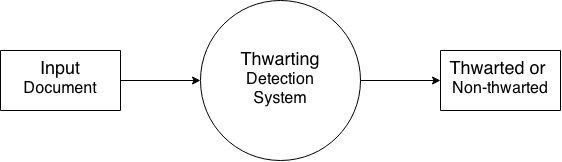
\includegraphics[scale=0.6]{gfx/flow.png}
\caption{Thwarting detection system }
\centering
\end{figure}


\vspace{8mm}

To handle this problem, an aspect level of analysis is required. If we treat out target as a combination of subtargets arranged in a hierarchical fashion (with the original entity as root)
, thwarting can be considered as the phenomenon of polarity reversal at a higher level of the hierarchy compared to the polarity at lower level. Thus, the proposed solution
starts with constructing a domain ontology of the system under consideration.

\vspace{8mm}

For example, if we are detecting turnarounds in movie reviews, we will have to find the ontology of a movie. This can be done manually as well as automated, using techniques
like Latent Dirichlet Allocation (LDA). LDA can learn the key features of a movie (e.g. cast, acting, music etc.) from a movie review corpus. If LDA misses out on some
features, human intervention may be required to provide the necessary components. The obtained list of all components should be then arranged into a proper hierarchy by a
human annotator.

\begin{figure}[t]
\centering
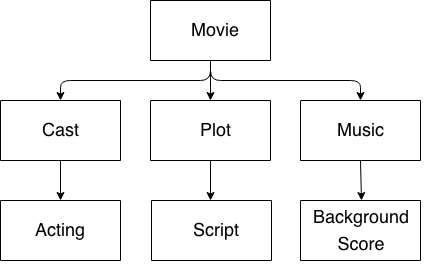
\includegraphics[scale=0.6]{gfx/onto.png}
\caption{Ontology creation for a movie - an example }

\end{figure}

The naive approach to detect thwarting after this would be to check the sentiment score obtained at all nodes in the ontology tree. If different levels exhibit different polarity,
the document is likely to be thwarted. In procedure, this is done in three distinct steps:

\begin{enumerate}[(a)]%for small alpha-characters within brackets.
\setlength{\itemsep}{15pt}
\item \textbf{Dependency parse: } For every input document, it has to undergo a dependency parsing first. This is essential to identify all the adjective-noun relations.

\item \textbf{Obtaining polarity at nodes: } Now, for all extracted nouns, we check if it is present in the domain ontology. If it is, the score for the corresponding node
will be the determined by the associated adjective word. 

\item \textbf{Thwarting detection: } Now that we have sentiment scores for all nodes in the ontology, we can summarize the sentiment polarity at each level of the ontology.
If there is a polarity reversal between levels, we can judge the document as thwarted.

\end{enumerate} 

\vspace{8mm}

However, this method fails to perform well in practical situations, since nodes at the same level may not be equally important for the sentiment of the document. For example,
For example, say in a camera ontology, the body and video capability might be subjective whereas any fault in the lens or the battery will render the camera useless, hence they are more critical.
Therefore, a relative weighing is required between all features of the ontology.

\vspace{8mm}

The idea used here is of percolated polarities. This means that polarity at a node is its polarity in the document along with the polarities of
all its descendants. This is based on the intuition that every word contributes some polarity to its parent node in the domain ontology. We can also define controlled
percolation, wherein the value added for a particular descendant is a function of its distance from the node.

\vspace{8mm}

For example,

\begin{framed}
$p(movie) = p(movie) + p(cast)/2 +p(plot)/2 + p(music)/2 + p(acting)/4 + p(script)/4 + p(background-score)/4$
\end{framed}

A more complicated approach involves using the above as preprocessing to obtain features and then pose the problem of thwarting detection as a classification problem. 
Ramteke et al. (2013) have used SVM classifier on such features to achieve an AUC score as high as 81\%.  \cite{puspak}

\section{Roadmap}

So far in this report, the importance of sentiment analysis as a research area has been established and its numerous applications stipulated. More importantly, it is shown why 
sentiment analysis is a challenging problem. In the chapters to follow, I have discussed some very useful approaches that may help in the direction of solving this problem of sentiment analysis
on text in general and on social media, in particular. Chapter 2 focuses on posing sentiment analysis as a classification problem and working out a machine learning based
solution to the problem at hand. Chapter 3 discusses the importance of social networks as a domain for applying sentiment analysis strategies and what are the special challenges there.
Lastly in Chapter 4, solutions specific to social media domain are discussed and it is demonstrated how we can utilise the power of social networks for obtaining better solutions
for our problem.
